\section{Gramáticas Formales}

\subsection{Definición}
Una \textbf{gramática formal} es un conjunto de reglas que describen la estructura de un lenguaje formal( si, otra forma). 
Se compone de un conjunto de símbolos terminales, un conjunto de símbolos no terminales, un símbolo inicial y un conjunto de reglas de producción. 
Las gramáticas formales se utilizan en el diseño de compiladores, análisis sintáctico y generación de lenguajes de programación

\begin{Def}
    Una \textbf{gramática formal} $G$ se define como un cuádruple $G = (\Gamma, \Sigma, P, S)$ donde:
    \begin{itemize}
        \item $\Gamma$ es un conjunto finito de \textbf{símbolos no terminales}.
        \item $\Sigma$ es un conjunto finito de \textbf{símbolos terminales} (alfabeto).
        \item $P$ es un conjunto de \textbf{reglas de producción} de la forma $A \rightarrow \alpha$, donde $A \in \Gamma$ y $\alpha \in (\Gamma \cup \Sigma)^*$.
        \item $S \in \Gamma$ es el \textbf{símbolo inicial}.
    \end{itemize}
\end{Def}

\textbf{Ejemplo:} Consideremos la gramática $G = (V, \Sigma, P, S)$ donde:
\begin{itemize}
    \item $V = \{S\}$
    \item $\Sigma = \{a, b\}$
    \item $P = \{S \rightarrow aSb \mid \lambda\}$
    \item $S$ es el símbolo inicial.
\end{itemize}

Otra manera de representar las reglas de producción es, :
\begin{align*}
    S &\rightarrow aSb \\
    S &\rightarrow \lambda
\end{align*}

También podemos escribir las reglas de producción en una sola línea, separando las diferentes producciones con el símbolo "|":
\begin{align*}
    S &\rightarrow aSb \mid \lambda
\end{align*}

O incluso usar otra notación alternativa, como la de Bakus Naur (BNF):
\begin{align*}
    <S> \ \ &::= a<S>b \mid \lambda
\end{align*}

\subsection{Tipos de Gramáticas}

Esta gramática genera el lenguaje $L(G) = \{a^n b^n \mid n \geq 0\}$, que consiste en cadenas de la forma $a^n b^n$ donde $n$ es un número entero no negativo. Las gramáticas formales se clasifican en diferentes tipos según su poder expresivo. La jerarquía de Chomsky clasifica las gramáticas en cuatro tipos:
\begin{itemize}
    \item \textbf{Gramáticas Tipo 0:} Gramáticas sin restricciones, que pueden generar cualquier lenguaje recursivamente enumerable.
    \item \textbf{Gramáticas Tipo 1:} Gramáticas sensibles al contexto, que generan lenguajes contextuales. (Libres de contexto)
    \item \textbf{Gramáticas Tipo 2:} Gramáticas libres de contexto, que generan lenguajes libres de contexto.
    \item \textbf{Gramáticas Tipo 3:} Gramáticas regulares, que generan lenguajes regulares.
\end{itemize}

Las reglas de producción cambian o tienen restricciones dependiendo del tipo de gramática. 
Por ejemplo, en las gramáticas regulares (Tipo 3), las reglas de producción tienen la forma $A \rightarrow wB$,
donde $A$ es un símbolo no terminal y $w$ es una cadena de símbolos terminales. Es decir, el lado derecho solo puede tener un símbolo no terminal. 

En las gramáticas regulares (Tipo 2) las reglas de producción tienen la forma $A \rightarrow (\Sigma \cup \Gamma)^*$, 
es decir, el lado derecho puede ser una combinación de símbolos terminales y no terminales. 

\begin{figure}
    \centering
    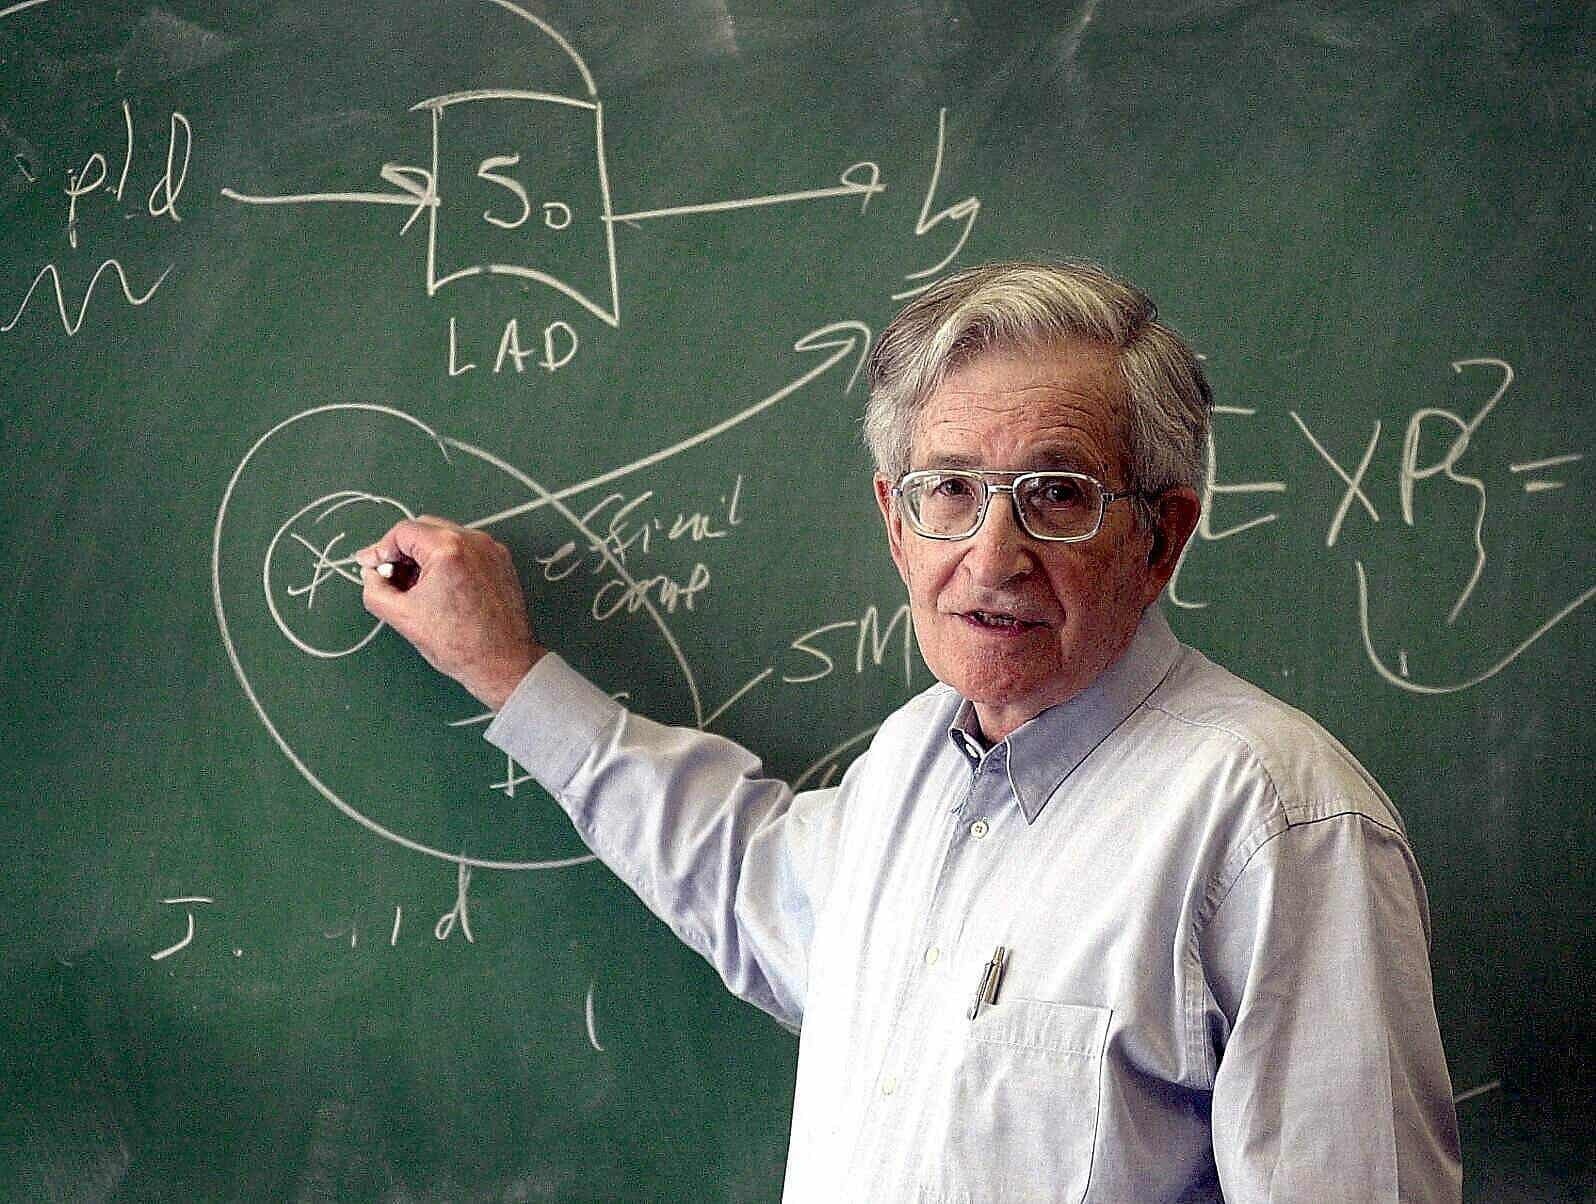
\includegraphics[width=0.5\textwidth]{images/chomsky-escribiendo.jpg}
    \caption{Noam Chomsky, escribiendo cosas de lenguajes}
\end{figure}

\begin{figure}
    \centering
    
\includegraphics[width=0.5\textwidth]{images/chomsky-vs-foucault.jpg}
    \caption{Chomsky vs Foucault, 1971. Ver debate completo sobre \href{https://www.youtube.com/watch?v=3wfNl2L0Gf8}{\textit{La naturaleza humana}}}
\end{figure}

Las reglas de producción son una función que toma símbolos no terminales y terminales y devuelve cadenas de símbolos terminales y no terminales. Formalmente se escribe como:

$$P: (\Gamma \cup \Sigma)^*  \Gamma (\Gamma \cup \Sigma)^* \rightarrow (\Gamma \cup \Sigma)^*$$

Vamos a desmenuzar un poco la definición.

\begin{itemize}
    \item $\Gamma$ es el conjunto de símbolos no terminales, que son los símbolos que pueden ser reemplazados por otros símbolos en las reglas de producción. En el ejemplo anterior, $S$ es un símbolo no terminal.
    \item $\Sigma$ es el conjunto de símbolos terminales, que son los símbolos que no pueden ser reemplazados por otros símbolos en las reglas de producción. En el ejemplo anterior, $a$ y $b$ son símbolos terminales.
    \item $(\Gamma \cup \Sigma)^*$ es el conjunto de todas las cadenas posibles que se pueden formar con los símbolos terminales y no terminales. El asterisco indica que puede haber cero o más repeticiones de los símbolos.
    \item $(\Gamma \cup \Sigma)^*  \Gamma (\Gamma \cup \Sigma)^*$ es el conjunto de todas las cadenas posibles que contienen al menos un símbolo no terminal. Esto es importante porque las reglas de producción solo pueden aplicarse a cadenas que contienen símbolos no terminales.
    \item La flecha $\rightarrow$ indica que la función de producción toma una cadena que contiene al menos un símbolo no terminal y la transforma en otra cadena que puede contener tanto símbolos terminales como no terminales.
\end{itemize}


\textbf{Ejemplo:} Consideremos la gramática $G = (V, \Sigma, P, S)$ donde:

\begin{align*}
    S &\rightarrow HOLA \\
    H &\rightarrow h \mid \lambda \\
    O &\rightarrow o \mid oO \\
    L &\rightarrow l  \\
    A &\rightarrow a \mid aA \mid i \mid iA \\
\end{align*}

Esta gramática genera el lenguaje $L(G) = \{ola,hola, holaa, holaaa, holi, holii, holiii \dots\}$, 
que consiste en cadenas que comienzan con \texttt{h} o sin \texttt{h}, seguido de una o más \texttt{o}, seguido de una \texttt{l}, 
y terminan con una o más \texttt{a} o \texttt{i}.

\subsection{Derivaciones y Lenguajes Generados}
\begin{Def}
    Decimos que una cadena $w \in \Sigma^*$ es \textbf{generada} por la gramática $G$ si existe una secuencia finita de aplicaciones de las reglas de producción que transforman 
    el símbolo inicial $S$ en la cadena $w$. Esta secuencia se llama una \textbf{derivación} de $w$ a partir de $S$.

    $$L(G) = \{ w \in \Sigma^* \mid S \Rightarrow^{*} w \}$$
\end{Def}

\textbf{Ejemplo:} Consideremos la gramática anterior y la cadena $w = \texttt{holaaa}$. Podemos derivar $w$ a partir de $S$ de la siguiente manera:

\begin{align*}
    S &\Rightarrow HOLA \\
    &\Rightarrow hOLA \\
    &\Rightarrow hoLA \\
    &\Rightarrow holA \\
    &\Rightarrow holaA \\
    &\Rightarrow holaaA \\
    &\Rightarrow holaaa
\end{align*}

Por lo tanto, $w$ es generada por la gramática $G$ y pertenece al lenguaje $L(G)$.

\begin{Def}
    Podemos hacer dos tipos de derivaciones \textit{especiales}, la derivación más a la izquierda y la derivación más a la derecha.
    \begin{itemize}
        \item Una \textbf{derivación más a la izquierda} es una derivación en la que en cada paso se reemplaza el símbolo no terminal más a la izquierda en la cadena actual.
        \item Una \textbf{derivación más a la derecha} es una derivación en la que en cada paso se reemplaza el símbolo no terminal más a la derecha en la cadena actual.
    \end{itemize}
\end{Def}

\text{Ejemplo:} Consideremos la gramática anterior y la cadena $w = \texttt{holaaa}$. Podemos derivar $w$ a partir de $S$ de la siguiente manera usando una derivación más a la derecha:

\begin{align*}
    S &\Rightarrow HOLA \\
    &\Rightarrow HOLaA \\
    &\Rightarrow HOLaaA \\
    &\Rightarrow HOLaaa \\
    &\Rightarrow HoLaaa \\
    &\Rightarrow hoLaaa \\
    &\Rightarrow holaaa
\end{align*}

Anteriormente habíamos mostrado la derivación más a la izquierda. 

\begin{Def}
    Una \textbf{forma sentencial} es cualquier cadena de símbolos terminales y no terminales que puede ser derivada del símbolo inicial $S$ mediante una secuencia finita de aplicaciones de las reglas de producción. Formalmente, una cadena $\alpha \in (\Gamma \cup \Sigma)^*$ 
    es una forma sentencial si existe una secuencia finita de derivaciones $S \Rightarrow^{*} \alpha$.
\end{Def}

\begin{Def}
    Una \textbf{sentencia} es una forma sentencial que consiste únicamente en símbolos terminales. Es decir, una cadena $w \in \Sigma^*$ es una sentencia si existe una secuencia finita de derivaciones $S \Rightarrow^{*} w$.
\end{Def}

\subsection{Árboles de Derivación y Ambigüedad}
\begin{Def}
    El arbol de derivación es una representación gráfica de una derivación en una gramática formal. Es un árbol donde:
    \begin{itemize}
        \item La raíz del árbol es el símbolo inicial $S$.
        \item Cada nodo interno representa un símbolo no terminal.
        \item Cada hoja representa un símbolo terminal.
        \item Las ramas representan las aplicaciones de las reglas de producción.
    \end{itemize}
\end{Def}

\textbf{Ejemplo:} Consideremos la gramática anterior y la cadena $w = \texttt{holaaa}$. El árbol de derivación para $w$ es:

\begin{center}
\begin{forest} for tree={
    edge path={\noexpand\path[\forestoption{edge}] (\forestOve{\forestove{@parent}}{name}.parent anchor) -- +(0,-12pt)-| (\forestove{name}.child anchor)\forestoption{edge label};}
}
[S
[H [h]]
[O [o]]
[L [l]]
[A [aA [aA [a]]]]]
\end{forest}
\end{center}

También podríamos ver la derivación de \texttt{ola}:

\begin{center}
\begin{forest} for tree={
    edge path={\noexpand\path[\forestoption{edge}] (\forestOve{\forestove{@parent}}{name}.parent anchor) -- +(0,-12pt)-| (\forestove{name}.child anchor)\forestoption{edge label};}
}
[S
[H [$\lambda$]]
[O [o]]
[L [l]]
[A [a]]]
\end{forest}
\end{center}

\begin{Def}
    Una gramática formal es \textbf{ambigua} si existe al menos una cadena en el lenguaje generado por la gramática que puede ser derivada de más de una manera distinta, es decir, que tiene más de un árbol de derivación diferente. O si 
    existen dos derivaciones izquierdas o derechas distintas para la misma cadena.
\end{Def}

Mientras que no existe un algoritmo general para determinar si una gramática es ambigua (es decir, el problema es indecidible), 
podemos mostrar que una gramática es ambigua proporcionando un ejemplo concreto de una cadena que tiene múltiples derivaciones o 
árboles de derivación distintos.

\subsection{Relación entre Gramáticas y Expresiones Regulares}

Otra cosa que podemos hacer es diseñar gramáticas a partir de expresiones regulares, de hecho las expresiones regulares son equivalentes a las gramáticas regulares. Por ejemplo, si tenemos la expresión regular $(0+1)^*1(0+1)$, 
podemos construir la siguiente gramática:
\begin{align*}
    S &\rightarrow A1B \\
    A &\rightarrow 0A \mid 1A \mid \lambda \\
    B &\rightarrow 0 \mid 1
\end{align*}

Y podemos incluir otras producciones para hacer la gramática estrictamente de tipo 3 (regulares).

Si queremos generar una o más repeticiones de un símbolo, podemos usar recursión de símbolo. 
Por ejemplo, para generar una o más repeticiones de $0$ ocupamos $0A$, para generar cero o más 
repeticiones de $0$ ocupamos $0A \mid \lambda$.
Para generar una o más repeticiones de $1$, ocupamos $1A$, y para cero o más repeticiones 
de $1$, ocupamos $1A \mid \lambda$. Entonces para representar 
$(0+1)^{*}$ ocupamos $A \rightarrow 0A \mid 1A \mid \lambda$.

\begin{align*}
    S &\rightarrow 0S \mid 1S \mid A \\
    A &\rightarrow 1B \\
    B &\rightarrow 0 \mid 1
\end{align*}






